\chapter{Theoretical Motivation} \label{chap-theory}

DGLAP
Higgs related to top
interaction lagrangian with effective operators
electric dipole moment and a top quark with 4/3 charge
anomolous couplings
talk about top quarks - different chapter maybe?

hard-scattering pp collisions
\begin{equation}
\sigma(pp \to X) = \int^1_0dx_1 \int^1_0dx_2 \sum_{a,b} f_a(x_1, \mu_F^2) f_b(x_2, \mu_F^2) \hat{\sigma}_{ab \to X}(Q^2, \mu_F^2)
\end{equation}

\section{The Standard Model of Particle Physics} \label{sec-StandardModel}

\subsection{Gauge theory}

Almost all of the physics within Standard Model arises directly from imposed symmetires. Interactions are produced by requiring local gauge invariance under specific symmetry groups. We define the Standard Model in group theory as the unification of two gauge symmetry groups, describing the electroweak and strong interactions. The Glashow-Weinberg-Salam electroweak model sees the electromagnetic and weak interactions combined to create the electroweak gauge symmetry group $SU(2)_L \otimes U(1)_Y$, where the gauge symmetry group for strong interactions is defined as $SU(3)_C$. Thus, we can define the gauge symmetry group of the Standard Model to be 

\begin{equation}
SU(3)_C \otimes SU(2)_L \otimes U(1)_Y.
\end{equation}

In order to explain the concept of gauge invariance we start by considering changes to the phase of the wavefunctions or fields. Let us take the Lagrangian density of a free Dirac field, $\psi$, describing all free-moving spin-$\frac{1}{2}$ fermions with a mass m:  

\begin{equation} \label{eqn-DiracLagrangian}
\lumi = \bar{\psi}(i \gamma^{\mu}\partial_{\mu}-m)\psi
\end{equation}

where $\gamma^{\mu}$ are the Dirac matrices. We can show that this is invariant under phase rotations, defined by

\begin{equation}
\psi \to \psi'= e^{i \theta}\psi, \quad \bar{\psi} \to \bar{\psi}' = e^{- i \theta}\bar{\psi},
\end{equation}

as the exponential factors will cancel each out, thus we have a $U(1)$ symmetry and corresponding conserved current. This is what is known as a global phase transformation due to the time dependency of $\theta$. However, we require a local gauge invariance, and therefore a local phase transformation must be applied such that $\theta$ is different at every space-time point, which we now define as $\theta (x_{\mu})$. The local phase transformations are applied to the wave function, $\psi$, and are defined in the following way:

\begin{equation}
\psi \to \psi'= e^{i \theta(x_{\mu})}\psi, \quad \bar{\psi} \to \bar{\psi}' = e^{- i \theta(x_{\mu})}\bar{\psi},
\end{equation} 

Dropping the space-time component $\mu$ from $x_{\mu}$ for simplicity, we can see that the Dirac equation is now not invariant under the local gauge transformation as

\begin{equation}
\partial_{\mu} (e^{i\theta(x)}\psi) = i(\partial_{\mu}\theta(x))e^{i\theta(x)}\psi + e^{i\theta(x)} \partial_{\mu}\psi 
\end{equation}

which we can then express in terms of the Lagrangian as

\begin{equation}
\lumi \to \lumi - [\partial_{\mu} \theta(x)] \bar{\psi} \gamma^{\mu} \psi.
\end{equation}

In order to restore local gauge invariance, we start by hypotheising that the fermions interact with a ``gauge field" $A_{\mu}$. We can then redefine our the interacting fermion Lagrangian 

\begin{equation} \label{eqn-DiracLagrangian}
\lumi = \bar{\psi}(i \gamma^{\mu}D_{\mu}-m)\psi
\end{equation}

where we replace the ordinary derivative, $\partial_{\mu}$ covariant derivative, $D_{\mu}$, defined as

\begin{equation}
\partial_{\mu} \to D_{\mu} = \partial_{\mu} + iqA_{\mu}.
\end{equation}

where

\begin{equation}
A_{\mu} \to A_{\mu} - \partial_{\mu} \theta (x).
\end{equation}

In this way the gauge transformation of the fields cancel with that of the fermion fields, and therefore invariance is restored. The Lagrangian of Equation \ref{eqn-DiracLagrangian} is exactly what we expect for a fermion in an electromagnetic field with charge q. The second term in the Lagrangian, $-q\bar{\psi}\gamma^{\mu}A_{\mu}\psi$, describes the interaction of a fermion with a vector field with coupling strength $q=Qe$, where Q is the charge of the particle in units of e, where e is the electromagnetic coupling constant. By forcing a local $U(1)$ gauge invariance, we have essentially introduced quantum electrodynamics (QED), with the exception of the gauge field (photon) kinematic term described by the field strength tensor, $F_{\mu \nu}$, denoted  

\begin{equation}
F^{\mu \nu} = \partial^{\mu}A^{\nu} - \partial^{\nu}A^{\mu}
\end{equation}

and thus we obtain the gauge-invariant QED Lagrangian density:

\begin{equation}
\lumi_{QED} = \bar{\psi}(i \slashed{D}_{\mu} - m) \psi - \frac{1}{4}F_{\mu \nu}F^{\mu \nu}
\end{equation}

where $\slashed{D}_{\mu}$ is equal to $\gamma^{\mu}(\partial_{\mu} + iqA_{\mu})$.

We note that the gauge field $A_{\mu}$ is required to be massless in order to satisfy invariance under a local gauge transformation. This property arises as the gauge field mass term $m^2A_{\mu}A^{\mu}$ would explicitly break the gauge invariance, and thus must be removed from the Lagrangian density. Therefore we can say that QED describes Dirac fields, such as electrons and positrons, interacting with Maxwell electromagnetic force fields, photons.

By requiring local gauge invariance of the Lagrangian density by introducing additional fields in order to make it covariant with respect to an extended group of local transformations, we describe the gauge principle that is a fundamental process in particle physics. For the case of QED, we have a group of $1 \times 1$ unitary matrices multiplied by the Dirac field. The set of transformations form the Lie group $U(1)$, a group that is commutative, and thus Abelian. Gauge principle or local gauge invariant transformations can be applied to any $SU(N)$ group; Chen Ning Yang and Robert Mills first produced a theory of the $SU(2)$ gauge group \cite{PhysRev.96.191}, which was later extended to an $SU(3)$ gauge group to create QCD.  

\subsection{The Electroweak Theory} \label{subsec-ElectroweakTheory}

A theory for the unification of the electromagnetic and weak forces was first proposed by the American physicist Sheldon Glashow in 1961 \cite{Glashow:1961tr} and was later independently revised by Steven Weinberg in 1967 \cite{PhysRevLett.19.1264} and Abdus Salam \cite{Salam:1959zz} with the introduction of massive vector bosons acquiring mass by the process of spontaneous symmetry breaking. The GSW electroweak model later saw the authors receive the Nobel prize in physics in 1979. The GSW electroweak theory requires a unification of the gauge groups $SU(2)_L \otimes U(1)_Y$, where the definition of the $U(1)$ group from the previous section now refers to the unitary group of $1 \times 1$ matrices with respect to the weak hypercharge, Y, defined as 

\begin{equation}
Q = I_W + \frac{Y}{2}
\end{equation}

where Q is the electric charge, and $I_W$ is the weak isospin, also denoted $I_3$. The weak force is the only force known to violate parity, and thus distinguish between right- and left-handedness and confirmed in 1957 \cite{PhysRev.105.1413}. We can thus define left-handed doublets and right-handed singlets for fermions as so

\begin{equation}
\begin{pmatrix}
u_L \\
d_L
\end{pmatrix}
,u_R,d_R;
\quad
\begin{pmatrix}
c_L \\
s_L
\end{pmatrix}
,c_R, s_R;
\quad
\begin{pmatrix}
t_L \\
b_L
\end{pmatrix}
,t_R, b_R;
\end{equation}

for each generation of quark, and

\begin{equation}
\begin{pmatrix}
\nu_{e,L} \\
e_L
\end{pmatrix}
,e_R;
\quad
\begin{pmatrix}
\nu_{\mu,L} \\
\mu_L
\end{pmatrix}
,\mu_R;
\quad
\begin{pmatrix}
\nu_{\tau,L} \\
\tau_L
\end{pmatrix}
,\tau_R;
\end{equation}

for each generation of leptons. 

Left-handed quark and lepton doublets have weak isospin values of $I_W = 1/2$ where the upper and lower particle in each have $I^3_W = +1/2$ and $-1/2$, respectively. Right-handed particles are defined as singlets under the $SU(2)_L \otimes U(1)_L$ gauge group symmetry and thus have weak isospin of $I_W = 0$. We define left- and right-handedness by applying projection operators to the fields, such that

\begin{equation}
\psi = \frac{1}{2}(1-\gamma^5)\psi + \frac{1}{2}(1+\gamma^5)\psi = \psi_L + \psi_R,
\end{equation}

where we define the $\gamma^5$ matrix as the product of all the gamma matrices

\begin{equation}
\gamma^5 = i\gamma^0 \gamma^1 \gamma^2 \gamma^3 = 
\begin{pmatrix}
0 & 1 \\
1 & 0
\end{pmatrix}
\end{equation}

such that $\left(\gamma^5\right)^2$ is equal to the $4 \times 4$ identity matrix.

% Gell-Mann 1964 \cite{GellMann:1964nj}

Analogous to the previous case describing the $U(1)$ electromagnetic gauge group, the full covariant derivative for the electroweak theory within a $SU(2)_L \otimes U(1)_L$ gauge symmetry is given by

\begin{equation}
\partial_{\mu} \to D_{\mu} = \partial_{\mu} - ig I_W \textbf{T}^i\textbf{W}^i_{\mu} - i\frac{g'}{2}YB
\end{equation}

The $g$ and $g'$ terms represent the coupling constants for the $SU(2)_L$ and $U(1)_Y$ gauge groups, respectively; $\textbf{T}^i$ represents the three generators of the $SU(2)_L$ gauge group defined by the Pauli matrices 

\begin{equation}
\sigma_1 = 
\begin{pmatrix}
0 & 1 \\
1 & 0
\end{pmatrix}
,
\quad
\sigma_2 =
\begin{pmatrix}
0 & -i \\
i & 0
\end{pmatrix}
,
\quad 
\sigma_3 = 
\begin{pmatrix}
1 & 0 \\
0 & -1
\end{pmatrix}. 
\end{equation}

$W^i_{\mu}$ are the gauge fields that are now introduced conserve invariance in the gauge symmetry group $SU(2)_L$; and $B$ is the new gauge field for the conservation of invariance in the $U(1)_Y$ gauge symmetry group. For right-handed particle singlets, the generators $\textbf{T}^i$ are equal to 0, and thus the second term in the electroweak covariant derivative vanishes, there we can define the electroweak Lagrangian density as such

\begin{equation}
\begin{split}
\lumi_{EWK} & = \bar{\psi}_L \gamma^{\mu} \left(i \i\partial_{\mu} - g I_W \textbf{T}^i \cdot \textbf{W}_{\mu} - \frac{g'}{2} Y B_{\mu}\right)\psi_L \\
& + \bar{\psi}_R \gamma^{\mu}\left(i \i\partial_{\mu} - \frac{g'}{2} Y B_{\mu}\right)\psi_R - \frac{1}{4}\textbf{W}_{\mu \nu}\textbf{W}^{\mu \nu} - \frac{1}{4} B_{\mu \nu} B^{\mu \nu} .
\end{split}
\end{equation}

Here we define $\psi_L$ and $\psi_R$ as the double and singlet fields. Although we introduce the gauge fields $\textbf{W}^i_{\mu} and B_{\mu}$ to conserve invariance, they have no direct physical relation to gauge bosons. Instead we combine the gauge fields to form physical gauge bosons in the following linear combinations:

\begin{align}
W^{\pm}_{\mu} & = \frac{1}{\sqrt{2}}(W^1_{\mu} \pm iW^2_{\mu}), \\
Z_{\mu} & = -B_{\mu}\sin\theta_W + W^3_{\mu}\cos\theta_W, \\
A_{\mu} & = B_{\mu}\cos\theta_W + W^3_{\mu}\sin\theta_W
\end{align}   

We form the physical fields of the $W^{\pm}$ and $Z^0$ bosons, and the photon ($A_{\mu}$) by the mixing of the $W^i_{\mu}$ and $B{\mu}$ gauge fields with respect to the weak mixing angle, $\theta_W$, where we define the electric charge as:

\begin{equation}
e = g'\cos\theta_W = g \sin\theta_W.
\end{equation}

At this point we have a theory of electroweak interactions that does not incorporate electromagnetism explicitly and where a the introduction of a mass term would explicitly break invariance of the $SU(2)$ and $U(1)$ symmetries, due to the way in which right- and left-handed fermions coupling differently. Therefore, all particles must be massless in this theory. We solve this problem via the process of spontaneous symmetry breaking in the Higgs mechanism, described in Section \ref{subsec-ElectroweakSymmetryBreaking}.  

\subsection{Quantum Chromodynamics} \label{subsec-QuantumChromodynamics}

assymptotic freedom David J. Gross and Frank Wilczek \cite{PhysRevD.8.3633}

H. David Polizer \cite{PhysRevLett.30.1346}

\begin{equation}
r = 
\begin{pmatrix}
r \\
b \\
g
\end{pmatrix}
\end{equation}


\begin{equation}
\lumi_{QCD} & = \bar{q}\left(\gamma^{\mu}\partial_{\mu} - m \right) q + g_s \left( \bar{q}\gamma^{\mu}T_a q \right) G^a_{\mu} - \frac{1}{4}G^a_{\mu \nu}G^{\mu \nu}_a
\end{equation}


\begin{equation} \label{equ-ckm}
\begin{pmatrix}
d' \\
s' \\
b' 
\end{pmatrix}
=
\begin{pmatrix}
V_{ud} & V_{us} & V_{ub} \\
V_{cd} & V_{cs} & V_{cb} \\
V_{td} & V_{ts} & V_{tb} 
\end{pmatrix}
\begin{pmatrix}
d \\
s \\
b 
\end{pmatrix}
\end{equation}

\begin{equation} \label{equ-ckm}
V_{CKM}
=
\begin{pmatrix}
0.97425 \pm 0.00022 & 0.2253 \pm 0.0008 & 0.00413 \pm 0.00049 \\
0.225 \pm 0.008 & 0.986 \pm 0.016 & 0.0411 \pm 0.0013 \\
0.0084 \pm 0.0006 & 0.040 \pm 0.0027 & 1.021 \pm 0.032} 
\end{pmatrix}
\end{equation}



\subsection{Electroweak Symmetry Breaking} \label{subsec-ElectroweakSymmetryBreaking}

Peter Higgs \cite{PhysRevLett.13.508}

Francois Englert and Robert Brout \cite{PhysRevLett.13.321}

\begin{equation}
\phi = 
\begin{pmatrix}
\phi^+ \\
\phi^0
\end{pmatrix}{
= \frac{1}{\sqrt{2}}
\begin{pmatrix}
\phi_1 + i \phi_2 \\
\phi_3 + i\phi_4
\end{pmatrix}
\end{equation}

\begin{equation}
\lumi_{Higgs} = (D_{\mu}\phi)^{\dagger}(D^{\mu}\phi) - V(\phi)
\end{equation}

\begin{equation}
V(\phi) = -\mu^2(\phi^{\dagger}\phi) + \lambda(\phi^{\dagger}\phi)^2
\end{equation}

\begin{figure}
\begin{center}
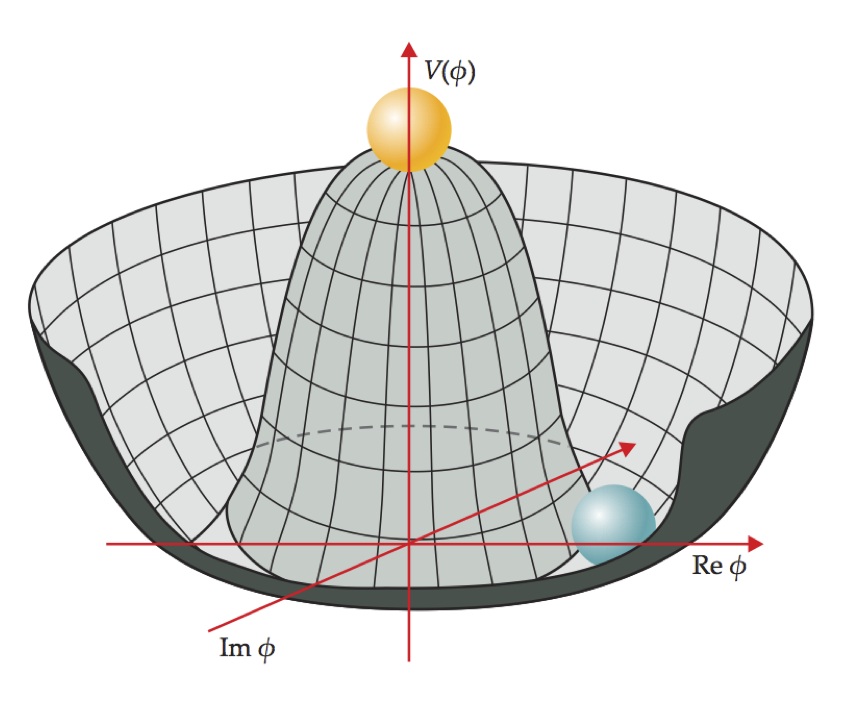
\includegraphics[width=0.7\textwidth]{Figures/MexicanHatPotential.png}
\caption{The ``Mexican Hat Potential" describing the vacuum expectation value of the Higgs in the real and imaginary planes, such that the minima lies below zero.}
\end{center}
\end{figure}

\begin{equation}
\braket{0|\phi|0} = \frac{1}{\sqrt{2}}
\begin{pmatrix}
0 \\
v
\end{pmatrix}
\end{equation}

\begin{equation}
\phi = \frac{1}{\sqrt{2}}
\begin{pmatrix}
0 \\
v + H
\end{pmatrix}
\end{equation}

\begin{equation}
\begin{split}
\lumi_{Higgs} & = \frac{1}{2}(\partial_{\mu}H)(\partial^{\mu}H) + \frac{1}{4}g^2 (H^2 + 2vH + v^2) W^+_{\mu} W^{-\mu} \\
& + \frac{1}{8} (g^2 + g'^2) (H^2 + 2vH + v^2) Z_{\mu} Z^{\mu} - \mu^2 H^2 - \frac{\lambda}{4} (H^4 + 4vH^3)
\end{split}
\end{equation}

\begin{figure}
\begin{center}
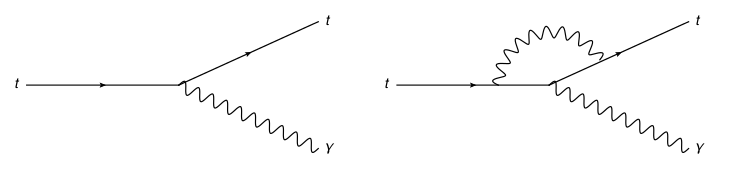
\includegraphics[width=\textwidth]{Figures/TopPhotonVertex.png}
\caption{Top-photon vertex. Left: Leading Order (LO). Right: One-Loop correction (NLO).}
\end{center}
\end{figure}

\begin{equation} \label{eqn-interactionlagrangian}
\lumi_{\gamma t\bar{t}} = -eQ_t\bar{t}\gamma^{\mu}tA_{\mu} - e\bar{t}\frac{i\sigma^{\mu\nu}q_{\nu}}{m_t}(d^{\gamma}_V+id^{\gamma}_A\gamma^5)tA_{\mu}
\end{equation}

\begin{equation}
\lumi^{eff.} = \Sum \frac{C_x}{\Lambda_x}O_x + ... ,
\end{equation}

\begin{align}\label{eqn-smparameterisations}
\delta d^{\gamma}_V = \frac{\sqrt{2}}{e}\text{Re}[c_WC^{33}_{uB\phi} + s_WC^{33}_{uW}]\frac{vm_t}{\Lamdba^2} \\
\delta d^{\gamma}_A = \frac{\sqrt{2}}{e}\text{Im}[c_WC^{33}_{uB\phi} + s_WC^{33}_{uW}]\frac{vm_t}{\Lamdba^2}
\end{align}

\begin{figure}
\begin{center}
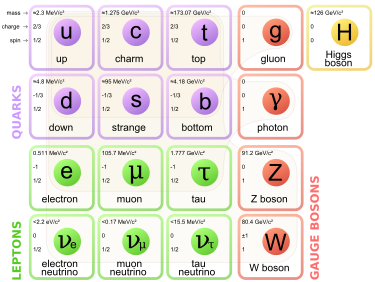
\includegraphics[width=0.8\textwidth]{Figures/StandardModel.png}
\caption{The Standard Model of particle physics.}
\end{center}
\end{figure}

\section{The Top Quark} \label{sec-TheTopQuark}

\begin{table} \label{tab:mumu_cutflow}
\begin{center}
\begin{tabular}{lccc}
\hline
\hline
\textbf{$\sqrt{s}$} & \textbf{$\sigma_{tot.}$} & \textbf{scales [pb]} & \textbf{pdf [pb]} \\
\hline
Tevatron 1.9 TeV & 7.164 & & \\
LHC TeV & 172.0 & $^4.4_5.8$ &  \\ 
LHC 8 TeV & 245.8 & & \\
LHC 14 TeV & 953.6 & & \\
\hline
\hline
\end{tabular}
\caption{\cite{Czakon:2013goa}}
\end{center}
\end{table}

\begin{figure} \label{fig-ttbarProductionLHC}
\begin{center}
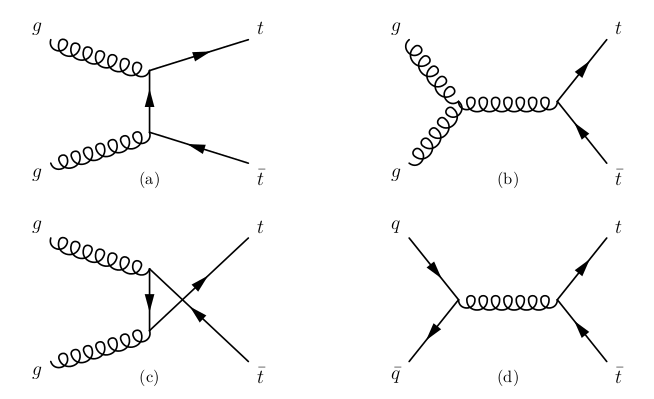
\includegraphics[width=\textwidth]{Figures/ttbarProductionLHC.png}
\caption{Lowest level diagrams for $t\bar{t}$ production at the LHC. Gluon scattering processes, {(a)}, {(b)}, and {(c)}, are the dominant processes at LHC energies, while quark scattering, process {(d)}, is the dominant one at TeVatron energies. \cite{SergeyThesis}}
\end{center}
\end{figure}

\begin{figure} \label{fig-singletopProductionLHC}
\begin{center}
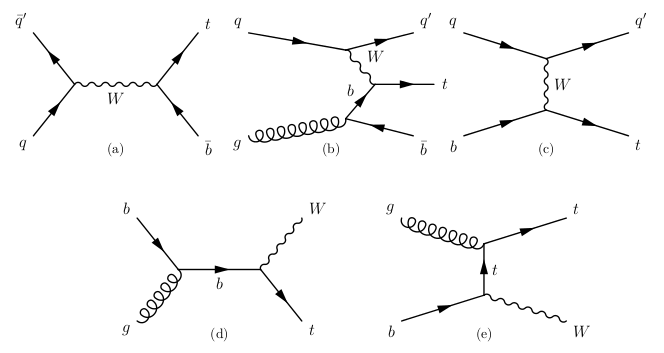
\includegraphics[width=\textwidth]{Figures/singletopProductionLHC.png}
\caption{Leading-order level diagrams for single top production at the LHC. {(a)} s-channel, {(b)} and {(c)} represent the t-channel, {(d)} and {(e)} both represent the two tW channels. \cite{SergeyThesis}}
\end{center}
\end{figure}

\begin{figure}
\begin{center}
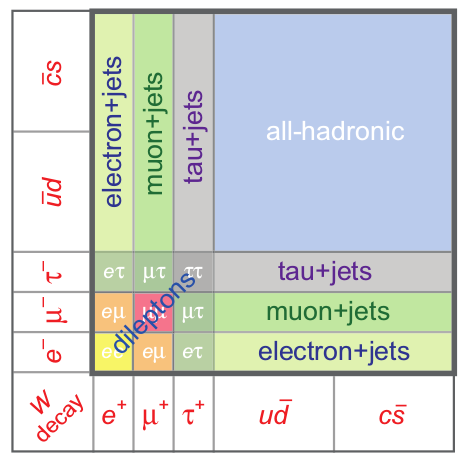
\includegraphics[width=0.5\textwidth]{Figures/ttbarDecayFractions.png}
\caption{Branching fractions of the W decays within top quark pairs. \cite{ttbarDecayFractions}}
\end{center}
\end{figure}

\begin{figure} \label{fig-ttgammaFeynmanDiagram}
\begin{center}
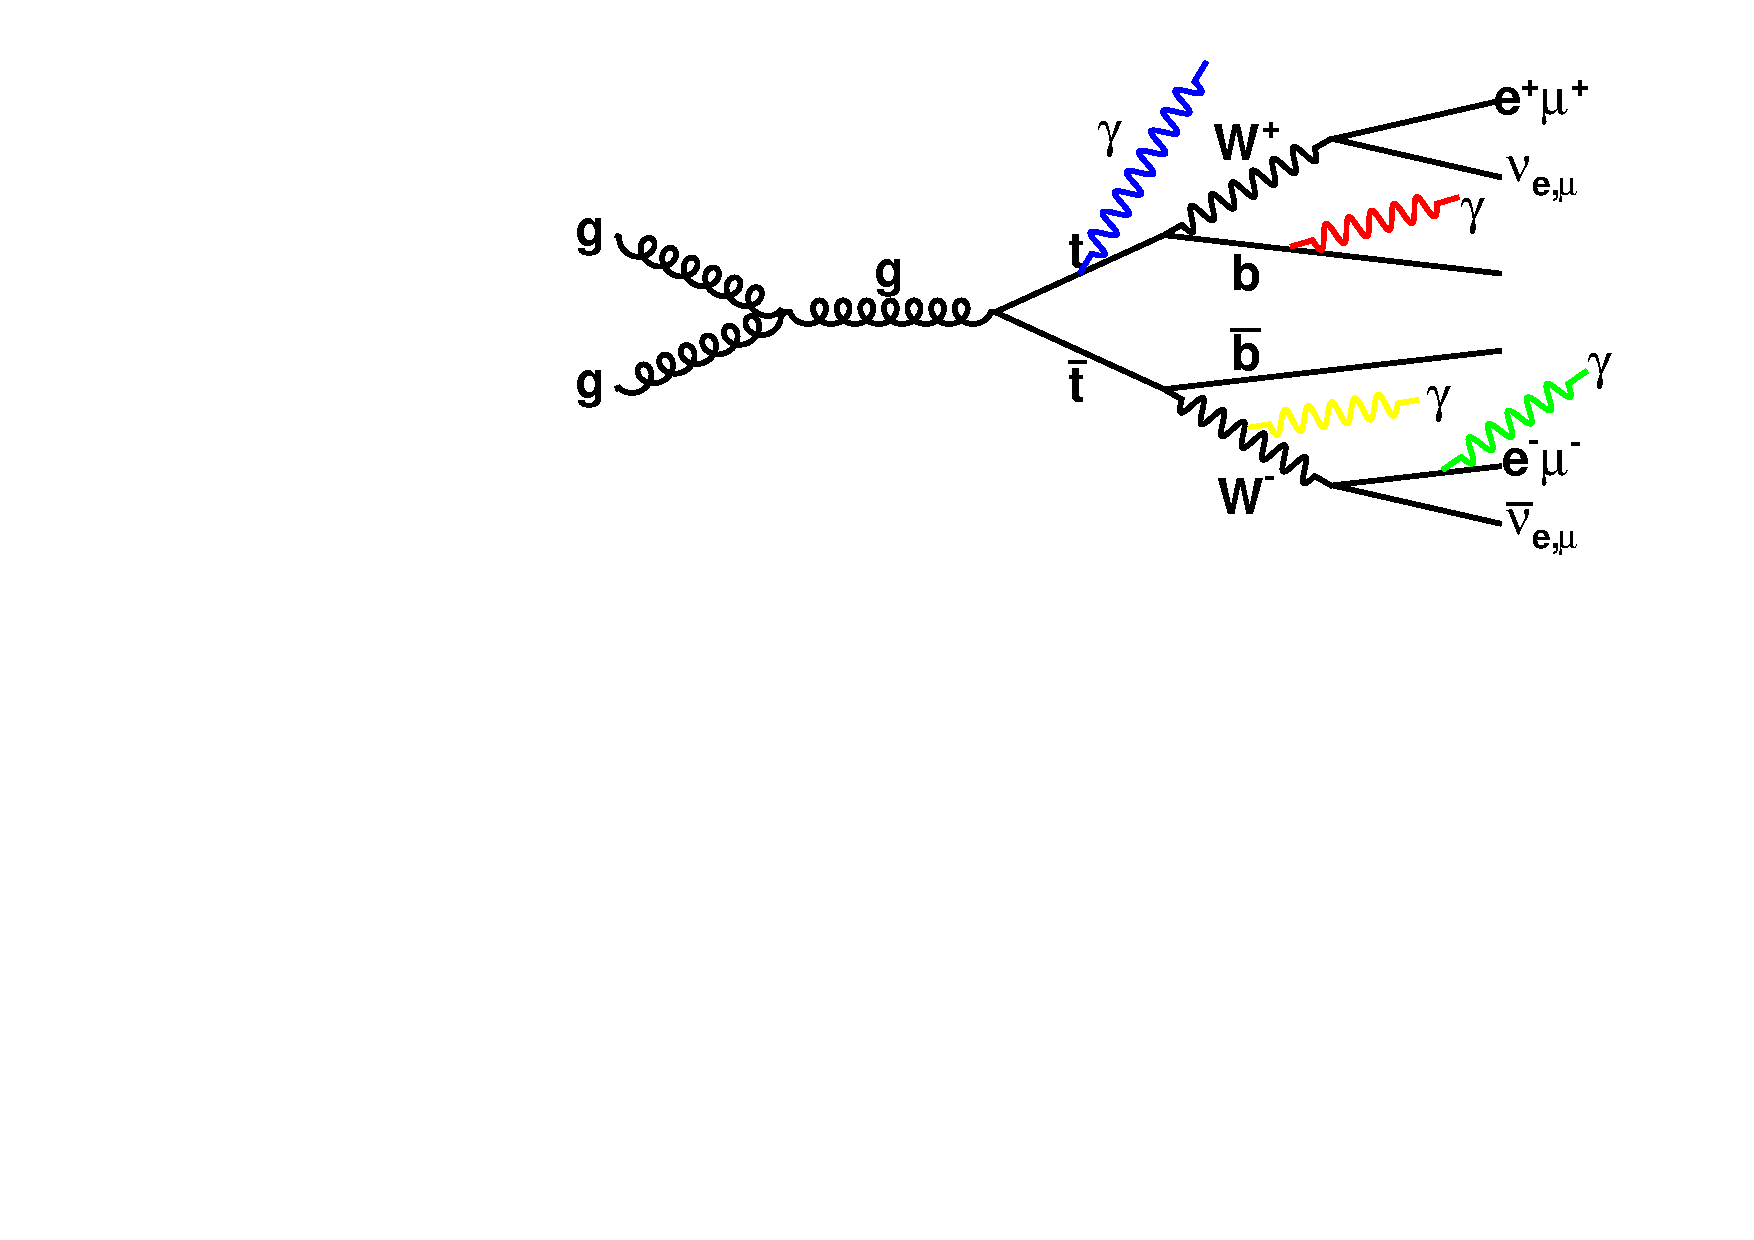
\includegraphics[width=0.9\textwidth]{Figures/ttgammaFeynmanDiagram.pdf}
\caption{}
\end{center}
\end{figure}